\documentclass[a4paper]{article}
\usepackage{graphicx}
\usepackage{amssymb}
\usepackage{amsmath}
\usepackage{bm}
\usepackage{color}
\usepackage{float}
\usepackage{bm}
\usepackage{physics}
\usepackage{subcaption}


\begin{document}

\section{Kalman Filter}

\subsection{How to update Kalman Filter}
Given a vector x which follow a gaussian probability distribution, the marginals and the conditions are gaussian distributions.

\subsubsection{Linear Model}
The Kalman filter assumes a linear transition and observation model with zero mean gaussian noise
\\
For the prediction state update:
$x_t = A_tx_{t-1} + B_tu_t + \epsilon_t$

\begin{itemize}
    \item The first term will take the previous state times a matrix
    \item The second term will take in the control commands
    \item The last term will encode covariance or uncertainty into the prediction step
\end{itemize}

For the measurement:
$z_t = C_tx_t + \delta_t$
\begin{itemize}
    \item Predicted observation based on the state
    \item $C_t$ will transform from the state space to the observation space
    \item $\delta_t$ is the noise
\end{itemize}

Matricies explained:
\begin{itemize}
    \item $A_t$ is an $(n,n)$ matrix which describes how the state evolves from t-1 to t without any controls or noise. More of the environmental factors like blowing wind or current velocity of the robot.
    \item $B_t$ is an $(n, l)$ matrix which describes how the control changes from state t-1 to t. l is the dimensionality of the control vector and this matrix can transform the odometry to the state measurement
    \item $C_t$ is an $(k, n)$ matrix which describes how to map the state $x_t$ to an observation $z_t$
    \item $\epsilon_t$ Represents the process noise at time t, refers to covariance $R_t$
    \item $\delta_t$ Represents the measurement noise, refers to covariance $Q_t$
\end{itemize}

\subsection{Deriving the Representation, $\mu$ and $\Sigma$}

\subsection{Kalman Filter Algorithm}
\begin{figure}
    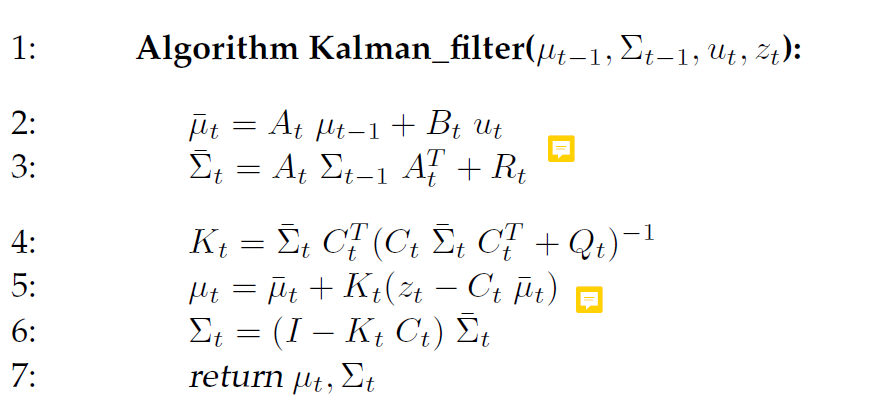
\includegraphics[width=0.9\textwidth]{KalmanAlgo.PNG}
\end{figure}

The predicted mean is just exploiting the linear model. The covariance is just an additive noise from the covariance matrix $R_t$

The correction step is essentially a weighted sum of the belief and the measurement. The weighting factor is called the \textbf{Kalman Gain}. The kalman gain will be high when the covariance is greater in the motion model or small in the measurement model. For the mean correction, kalman gain turns out to be the weight of the residual for the observation/measurement which is really just how much should I trust the measurement I just made when correcting the mean. The covariance correction also uses the kalman gain

\end{document}